\documentclass{exam}
\usepackage{mainExam}

\title{Correction du Contrôle}
\date{23 Mai 2024}
\author{Seconde 9}

\firstpageheader{Nom : }{}{Exercice choisi : }

\begin{document}
\maketitle
\thispagestyle{head}
\begin{questions}
\question Résoudre sur $\R$ les inéquations suivantes, en donnant l'ensemble des solutions sous la forme d'un intervalle. 
\begin{parts}
\part $3x - 7 \geq 4$
\part $-8x - 13 \geq 4x + 11$
\end{parts}
\vspace*{1cm}
\question Soit une fonction $f$ dont la courbe représentative $\mathcal{C}_f$ est donnée par la figure ci-contre.
\begin{center}
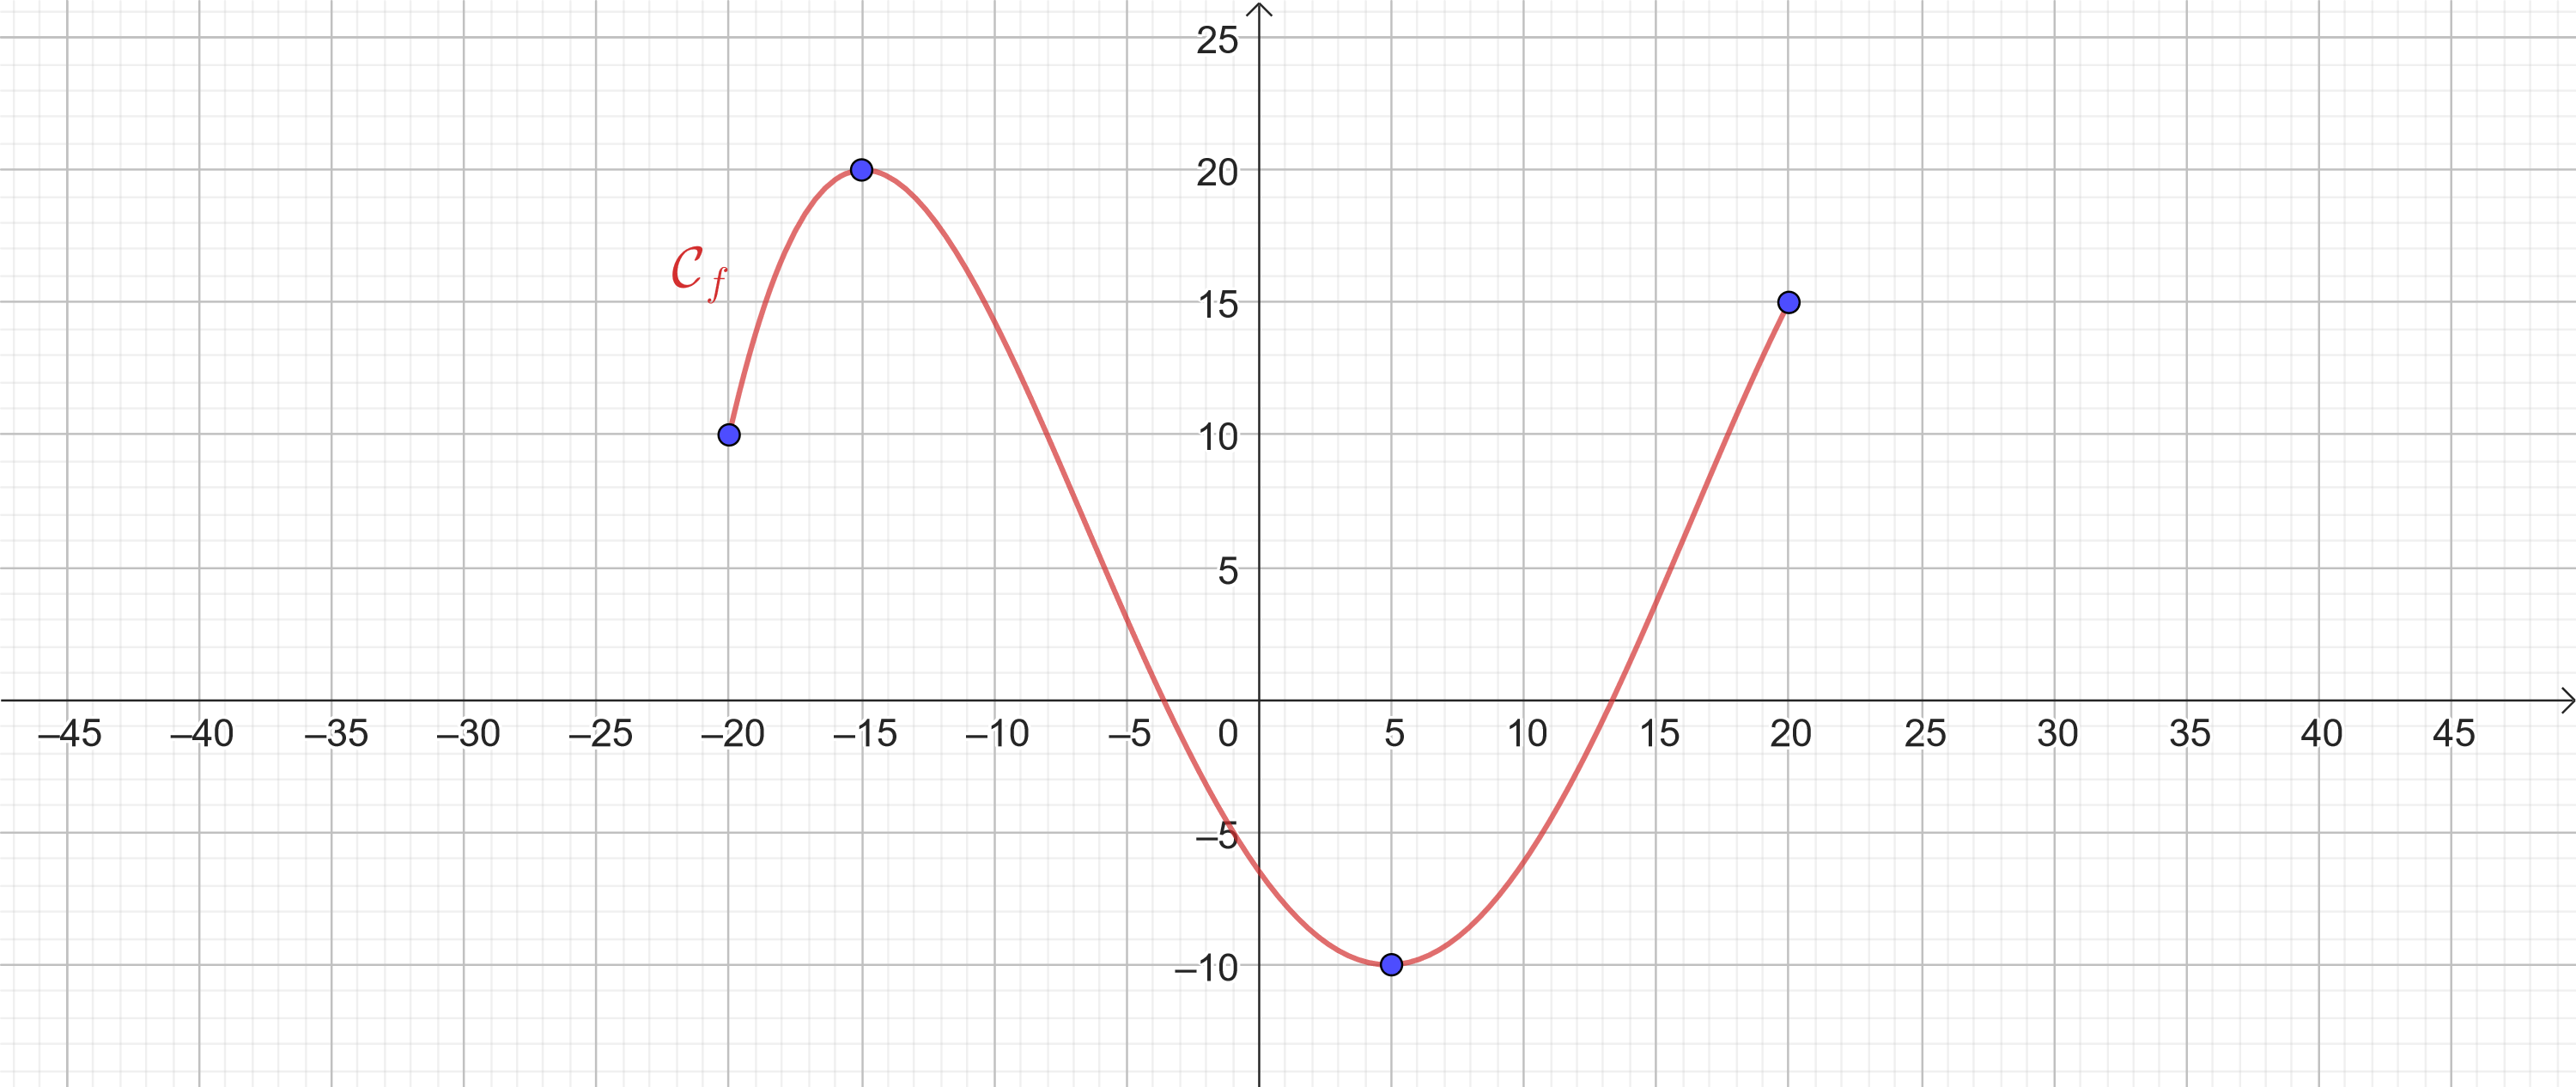
\includegraphics[width=0.9\textwidth]{Courbe1.png}
\end{center}
\begin{parts}
\part Quel est l'ensemble de définition de la fonction $f$ ?
\part Donner son maximum et son minimum.
\part En quelles valeurs la fonction $f$ atteint-elle son maximum et son minimum ?
\part Compléter le tableau de variation de la fonction $f$.
\begin{center}
\begin{tikzpicture}
\tkzTabInit{$x$ / 0.5, Variations de $f$ / 2}{,,};
\end{tikzpicture}
\end{center}
\end{parts}
\vspace*{1cm}
\question Soient deux points $A(16 + t;12 - t)$ et $B(4;6+2t)$ pour $t$ un nombre réel.
\begin{parts}
\part Calculer la distance $AB$ quand $t = -3$.
\part Exprimer la distance $AB$ en fonction de $t$.
\end{parts}
\newpage
\question Camille souhaite mesurer la température extérieure durant toute une journée. Elle installe un thermomètre capable de mesurer et de tracer la courbe de la fonction $h(t)$ donnant la température (en \unit{\celsius}) en fonction du temps $t$ (en heures).
\begin{parts}
\part Camille constate que le moment le plus chaud de la journée a été à 15 heures, et que la température a été la plus basse à deux moments différents. Compléter un tableau de variation probable pour la fonction $h$.
\begin{center}
\begin{tikzpicture}
\tkzTabInit{$x$ / 0.5, Variations de $f$ / 2}{,,};
\end{tikzpicture}
\end{center}
\part En déduire une courbe représentative pour $h(t)$, telle que les températures de l'après-midi sont plus chaudes que les températures du matin.
\end{parts}
\vspace*{1cm}
\question Soit $f$ une fonction à la fois paire et impaire. Donner la valeur de $f(1)$, $f(2)$ et $f(3)$.
\end{questions}
\end{document}
